\begin{frame}[ctb!]
  \frametitle{Engine : Parent-Child Relationship and Time Steps}
  In the Cyclus Engine, Models communicate messages and commands through their 
  parent-child relationship.
  \begin{itemize}
    \item all models have parents
    \item all children are 'owned' by their parent
    \item the region-institution-facility relationship is modeled through this relationship
  \end{itemize}
  Simulation time steps are decomposed into:
  \begin{itemize}
    \item tick: system requirements determined
    \item resolve: optimized solution of requirements found
    \item tock: solution executed
  \end{itemize}
\end{frame}

\begin{frame}[ctb!]
  \frametitle{Engine : Black-Box Paradigm}
  Facilities are treated as black boxes, i.e. only what comes in and
  out is recorded.
  \begin{itemize}
    \item facilities can be thought of as nodes: sources, sinks, or intermediaries
    \item material is passed between resources as a combination of:
      \begin{itemize}
        \item commodities (e.g. fresh/spent fuel)
        \item recipes (e.g. 51 GWd/tHM burnup)
        \item quantity
      \end{itemize}
  \end{itemize}
  \begin{figure}[htbp!]
    \begin{center}
      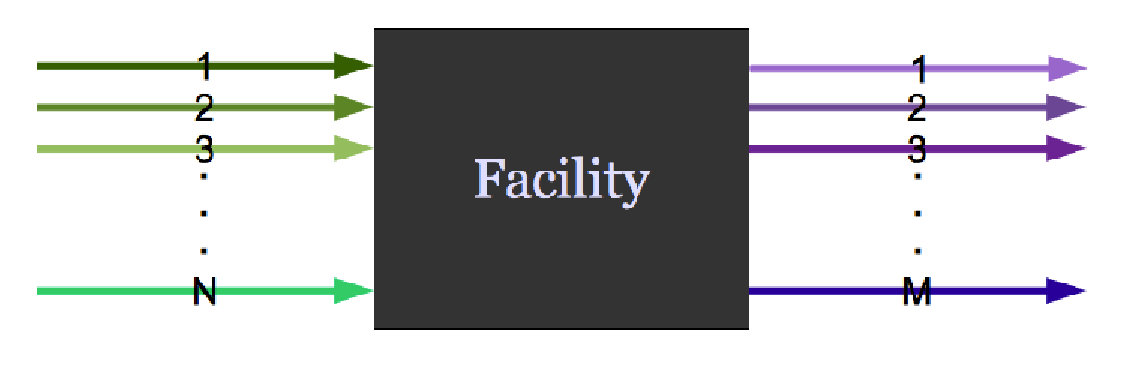
\includegraphics[height=3cm]{facility.eps}
    \end{center}
    \caption{Facilities are Black Boxes} 
    \label{fig:facility}
  \end{figure}
\end{frame}
